\documentclass[11pt]{article}
\usepackage[utf8]{inputenc}
\usepackage{listings}
\usepackage{graphicx}
\usepackage{amssymb}
\usepackage{amsmath}
\usepackage{colortbl}
\usepackage{algpseudocode}
\usepackage{algorithm}
\usepackage{subcaption}
\usepackage{amsfonts}

\title{RAPPORT : Projet Flood Filling}


\begin{titlepage}
\newcommand{\HRule}{\rule{\linewidth}{0.5mm}} 
\center

\includegraphics[width=9cm]{./img/logoenseirb.png}\\[1cm] 
\center 
\textsc{\LARGE ENSEIRB-MATMECA}\\[1.5cm] 
\textsc{\Large Filière Informatique, 1 ére année} 
\makeatletter
\HRule \\[0.4cm]
{ \huge \bfseries \@title}\\[0.4cm] 
\HRule \\[1.5cm]
 
\begin{minipage}{0.4\textwidth}
\begin{flushleft} \large

\textbf{Auteurs :}\\
- Abibi Aymane\\
- El bousty Badreddine\\
- Naami Anas\\
- Soufary Farouk\\
\end{flushleft}
\end{minipage}
~
\begin{minipage}{0.4\textwidth}
\begin{flushright} \large

\end{flushright}
\end{minipage}\\[2cm]
\makeatother
\end{titlepage}

\begin{document}

\newpage
\tableofcontents


\newpage
\section{Introduction}

%Ce compte-rendu est réalisé dans le cadre de notre formation en filière informatique à l'ENSEIRB-MATMECA. Il présente notre projet du 6-ème semestre et a pour objectif de mettre en pratique les enseignements dispensés en cours de programmation fonctionnelle, algorithmique des graphes, atelier algorithmique et programmation impérative . 
%Nous avons travaillé par groupe de 4 et été encadrés dans ce projet par Monsieur Popov Mihail. 

%Notre projet consiste à créer un jeux Flood-filling. Comme Flood-it, ce sont des jeux des stratégies qui est composé d'une grille de couleurs, et deux joueurs qui essaie de gagner la partie en propageant chacun une couleur de son choix en suivant quelque règle qui définit l'interdiction ou non de la couleur choisit. 
%
Dans le cadre du projet de programmation impérative du deuxième semestre, nous étions amenés à programmer en langage C afin d'atteindre l'ultime objectif du sujet, à savoir, faire tourner une partie du jeu Flood Filling entre deux joueurs. Des contraintes nous ont été données, mais aussi bon nombre de libertés. Parmi ces contraintes, nous citons par exemple l'utilisation d'une interface serveur-client, l'utilisation des bibliothèques dynamiques pour représenter les joueurs et la représentation des grilles du jeu par des graphes en utilisant d'abord des matrices creuses de la bibliothèque GSL comme des matrices d'adjacence pour ensuite les transformer en des matrices factorisées CSR.\\


Afin d'atteindre notre objectif dans ce projet, nous étions obligé de répartir les tâches entre les différents membres du groupe. Le travail a été décomposé en 4 sous objectifs essentiels à savoir :
\begin{itemize}
    \item Créer le support du jeu (graphes, coloration)
    \item Créer un serveur faisant tourner la partie
    \item Créer des bibliothèques dynamiques pour les joueurs
    \item Propager une couleur choisie par un joueur tout en respectant les règles du jeu
    \item Implémenter des stratégies pour les joueurs
\end{itemize}

Ce compte-rendu présente ainsi un résumé recouvrant le plus possible les réalisations majeures et les choix qui ont été discutés, décidés et implémentés par les différents membres du groupe.

% Image 
%
\section{Description générale du jeu Flood Filling}

La partie commence avec deux joueurs, leurs positions de départ sont différentes. Les couleurs choisies par le joueur lui font nécessairement gagner des cases (augmenter son score), et n'appartiennent pas à un ensemble de couleurs interdites défini au début de la partie.\\
La partie se termine si les deux joueurs choisissent de passer leur tour successivement (ils choisissent de jouer \texttt{NO\_COLOR}). Le gagnant est celui qui possède le plus de cases, et un joueur ne respectant pas l'une de ces règles est déclaré perdant.\\
\begin{figure}[h!]
    \begin{center}
        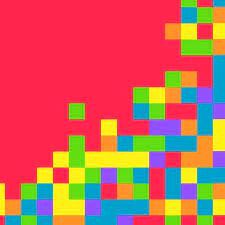
\includegraphics[scale=0.4]{./img/flood_it.jpeg}
    \end{center}
\end{figure}
\newline 
Les objectifs de ce projet sont détaillés ci-dessous :\\
\begin{itemize}
\item Pouvoir implémenter un ensemble de règles qui font jouer deux joueurs une partie, ainsi que des contraintes limitant les mouvements de chaque joueur.
% \item On doit tout d'abord pouvoir créer une grille de différentes types qui contient des cellules de couleurs générées de la manière de notre choix. 
\item Puis on doit pouvoir implémenter un ensemble de clients qui jouent d'une façon automatique sur leurs propre grille, et qui peuvent interagir entre eux à l'aide d'un serveur contenant la grille originale et qui donne à chacun son coup.
\item Implémenter un ensemble de règles et de stratégies et des algorithmes permettant la propagation des couleurs en prenant en considération les couleurs interdites pour chaque joueur : c'est la partie où on doit gérer les conflits.
\item Effectuer un ensemble de tests permettant de valider nos algorithmes et de faire jouer nos joueurs avec des stratégies différentes.
\end{itemize}

\section{Architecture du code et démarches suivies}
\newpage
\subsection{graphe de dépendances}
\begin{figure}[h!]
    \centering
    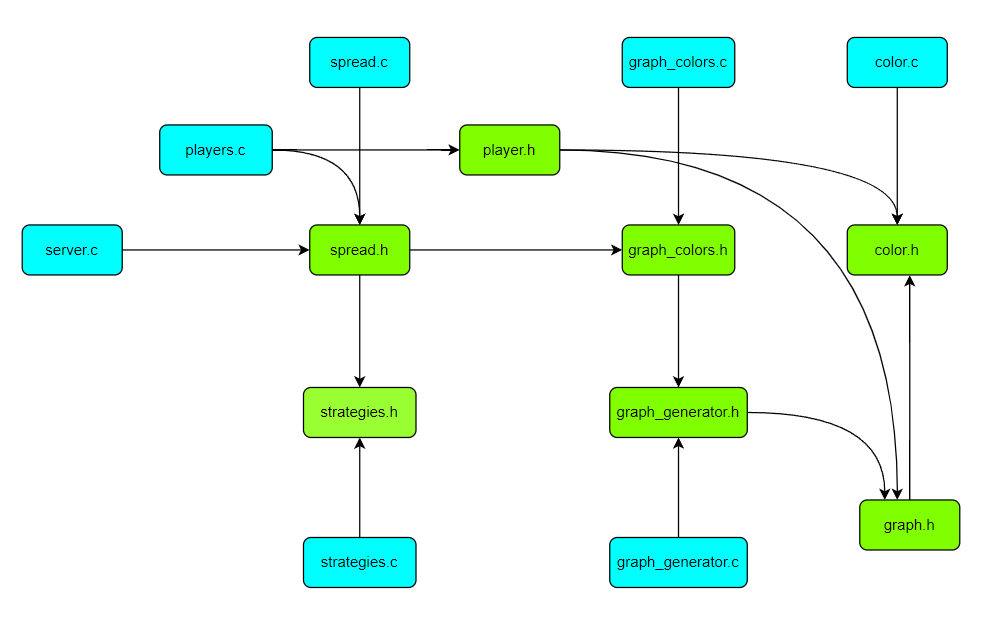
\includegraphics[scale=0.5]{img/graphe_dependance.png}
    \caption{Graphe de dépendances}
    \label{fig:grpahe_dep}
\end{figure}
\subsection{Générateur de graphes et couleurs}
\paragraph{\underline{Générateur de graphes:}\\\\}
Jouer au Flood-Filling nécessite d'implémenter un certain nombre de graphes. Quatre types ont été implémenter : \texttt{SQUARE}, \texttt{HGRAPH}, \texttt{DONUT}, \texttt{TORUS}.\\ 

Tout d'abord, les graphes sont définis en tant qu'une structure de données contenant un nombre de sommets \texttt{n}, une matrice d'adjacence de taille $\texttt{n.n}$ et un tableau contenant la position de départ de chaque joueur : \\
\begin{figure}[h!]
    \centering
    \begin{lstlisting}[language=C]
        struct graph_t {
            size_t num_vertices;
            gsl_spmatrix_uint* t;
            size_t positions[NUM_PLAYERS];
        }
    \end{lstlisting}
\end{figure} 
\newpage
Les valeurs de la matrice d'adjacence sont des binaires, si les sommets \textt{i} et \texttt{j} sont alors \texttt{t[i,j] = 1} sinon \texttt{t[i,j] = 0}. \\ \\
\big{\textbf{Exemple: SQUARE GRID\\}}
\newline
\begin{figure}[h!]
    \centering
    \begin{tabular}{|c|c|c|}
        \hline
        1\cellcolor{white} & 2\cellcolor{white} & 3\cellcolor{white}  \\
         \hline
         4\cellcolor{white} & 5\cellcolor{white} & 6\cellcolor{white}  \\
         \hline
         7\cellcolor{white} & 8\cellcolor{white} & 9\cellcolor{white}  \\
         \hline
    \end{tabular}
     $\Longrightarrow$
    $\begin{pmatrix}
        0 & 1 & 0 & 1 & 0 & 0 & 0 & 0 & 0 \\
        1 & 0 & 1 & 0 & 1 & 0 & 0 & 0 & 0 \\
        0 & 1 & 0 & 0 & 0 & 1 & 0 & 0 & 0 \\
        1 & 0 & 0 & 0 & 1 & 0 & 1 & 0 & 0 \\
        0 & 1 & 0 & 1 & 0 & 1 & 0 & 1 & 0 \\
        0 & 0 & 0 & 1 & 0 & 0 & 0 & 1 & 0 \\
        0 & 0 & 0 & 0 & 1 & 0 & 1 & 0 & 1 \\
        0 & 0 & 0 & 0 & 0 & 1 & 0 & 1 & 0 \\
    \end{pmatrix}$
\end{figure}
\newline
Après avoir implémenté les types cités précédemment, la génération des graphes de notre choix se fait à l'aide de la fonction \texttt{graph\_init} où on alloue dynamiquement la mémoire nécessaire. 
\begin{figure}[h!]
    \begin{lstlisting}[language=C]
        struct graph_t *graph_init(int num_vertices,
                                enum graph_type_t type);
    \end{lstlisting}
\end{figure}
La bibliothèque \texttt{GSL} offre la possibilité de créer des matrices creuses \texttt{COO} et \texttt{CSR}. Il s'avère qu'il est plus coûteux d'itérer sur une matrice \texttt{COO} que celle de type \texttt{CSR} , donc la fonction \texttt{graph\_compressed\_init} transformera la matrice du graphe retourner par \texttt{graph\_init} en une matrice \texttt{CSR}, ainsi on pourra la manipuler avec beaucoup plus de fluidité.
\paragraph{\underline{Générateur de couleurs:}\\\\}
En se limitant que sur huit couleurs définit par \texttt{color\_t}:  \\
\begin{figure}[h!]
    \centering
    \begin{lstlisting}[language=C]
        enum color_t {
            BLUE=0, RED=1, GREEN=2, YELLOW=3,
            ORANGE=4, VIOLET=5, CYAN=6, PINK=7,
            MAX_COLOR=8, NO_COLOR=-1
        };
    \end{lstlisting}
\end{figure}
\newline
De la même manière, la génération des couleurs nécessite des types de génération; RANDOM, CYCLIQUE, SYMÉTRIQUE.\\  
\begin{figure}[h!]
    \centering
    \begin{minipage}[c]{.2\linewidth}
        \begin{tabular}{|c|c|c|}
            \hline
            1\cellcolor{blue} & 2\cellcolor{yellow} & 3\cellcolor{green}  \\
            \hline
            4\cellcolor{blue} & 5\cellcolor{red} & 6\cellcolor{cyan}  \\
            \hline
            7\cellcolor{cyan} & 8\cellcolor{green} & 9\cellcolor{green}  \\    
            \hline
        \end{tabular}
        \caption{\\Random}
    \end{minipage}
    \begin{minipage}[c]{.2\linewidth}
        \begin{tabular}{|c|c|c|}
            \hline
            1\cellcolor{blue} & 2\cellcolor{red} & 3\cellcolor{green}  \\
            \hline
            4\cellcolor{yellow} & 5\cellcolor{magenta} & 6\cellcolor{cyan}  \\
            \hline
            7\cellcolor{blue} & 8\cellcolor{red} & 9\cellcolor{green}  \\    
            \hline
        \end{tabular}
        \caption{\\Cyclique}
    \end{minipage}
    \begin{minipage}[c]{.2\linewidth}
        \begin{tabular}{|c|c|c|}
        \hline
        1\cellcolor{blue} & 2\cellcolor{red} & 3\cellcolor{green}  \\
        \hline
        4\cellcolor{red} & 5\cellcolor{green} & 6\cellcolor{red}  \\
        \hline
        7\cellcolor{green} & 8\cellcolor{red} & 9\cellcolor{blue}  \\    
        \hline
        \end{tabular}
        \caption{\\symétrique}
    \end{minipage}
\end{figure}
\newline
Ensuite, on associe à chaque graphe un tableau de couleurs qui sera généré en fonction du type choisi grâce à la fonction \texttt{colors\_init}.

\begin{figure}[h!]
    \begin{lstlisting}[language=C]
        enum color_t * colors_init(struct graph_t * graph, 
                                enum color_type_t type_color, 
                                int num_colors);
    \end{lstlisting}
\end{figure}

\subsection{Implémentation des joueurs}
Les joueurs sont implémentés comme un ensemble de fonctions qui gère l'interaction avec le serveur. Dans le fichier de chaque joueur, on déclare globalement, un \texttt{id} qui désigne le joueur au serveur, un graphe, un tableau de couleur et un tableau de couleurs non permises qu'on appelle tableau de \texttt{forbidden}. la copie du tableau de couleur va être mise à jour au fur et à mesure, de l'évolution de la partie.
\par
Chaque joueur dispose de quatre fonctions :
\begin{itemize}
    \item \texttt{player\_get\_name} : retourne le nom du joueur.
    \item \texttt{initialize} : prend en paramètre un $id$, un graphe, tableau de couleurs, tableau de \texttt{forbidden}. Cette fonction copie les paramètres de la fonction dans les variables définies globalement dans le fichier. Ces paramètres constituent un environnement locale du joueur permettant de suivre la progression du jeu, et de fournir les coups qu'il veut jouer.
    \item \texttt{play} : prend en paramètres le coup joué par l'adversaire pour mettre à jour son propre tableau de couleur et calculer selon sa stratégie un coup qui va être retourner par la fonction.
    \item \texttt{finalize} : libère le graphe et le tableau de couleurs donnés aux joueurs par \texttt{initialize}.
\end{itemize}
\subsection{Serveur}
\par
L'implémentation du jeu nécessite une interaction serveur-clients. Le serveur connecte les joueurs, assure le bon déroulement du jeu, garantie qu'aucun joueur ne triche, et met à jour la grille du jeu pour chaque joueur.\\


\par
Le serveur alloue dynamiquement un graphe, un tableau de couleurs, ainsi qu'un tableau \texttt{forbidden} des couleurs interdites aux joueurs. Le serveur alloue une copie de graphe, une copie de tableau de couleurs, et une copie de tableau \texttt{forbidden} à chaque joueur. Ces copies seront passés aux joueurs en utilisant la fonction \texttt{initialize}.\\


\par
Les joueurs appliquent leurs coups sur les copies fournies par le serveur et informe le serveur du coup choisi par le biais de la fonction \texttt{play}, si le coup vérifie les 3 conditions: n'appartient pas au tableau \texttt{forbidden}, ne connecte pas les deux territoires et augmente le territoire du joueur, le serveur applique ce coup sur la grille principale et l'envoie au prochain joueur.\\


\par
Les clients sont chargés sous forme de bibliothèque dynamique et contiennent les mêmes noms de fonction, l'édition des liens qui se fait au moment de compilation n'est pas suffisante pour gérer les tours de rôle pour chaque joueur. La gestion des tours ainsi que l'interaction entre le serveur et les clients se fait à l'aide des fonctions de la bibliothèques \texttt{dlopen}, qui ouvre et prépare une bibliothèque partagée pour l'utilisation. Dans le cas où les deux joueurs, deux bibliothèques sont utilisées, on les charge dynamiquement en utilisant un tableau de longueur NUM\_PLAYERS, en occurrence 2:
\begin{figure}[h!]
    \begin{lstlisting}
        void handle[NUM_PLAYERS] = {dlopen("libplayer1.so")
                                ,dlopen("libplayer2.so")}
    \end{lstlisting}
    \caption{Tableau handle qui ouvre et prépare les bibliothèques utilisées}
    \label{fig:handle}
\end{figure}
\\


Le \textit{handle} retourné par chaque \texttt{dlopen}, est un chargement dynamique de fichiers passé en paramètre, pour importer donc les fonctions dans un \textit{handle}, on utilise la fonction \texttt{dlsym}.\\
\par


Ce mécanisme de chargement des fonction au besoin permet au serveur de bien gérer les tours de rôle, en accédant à chaque handle dans la tableau \ref{fig:handle}.\\
\par


La partie se termine si le serveur n'arrive pas à propager la couleur choisie par un joueur, ou si les deux joueurs choisissent de passer leur rôle successivement. Le score est calculé à la fin de la partie pour déterminer le joueur gagnant.\\
\par


Après la fin de la partie, on libère le graphe, le tableau de couleur, ainsi que le tableau \texttt{forbidden}, on libère aussi les copies données à chaque joueur en utilisant la fonction \texttt{finalize} puis on arrête le chargement des bibliothèques en utilisant la fonction \texttt{dlclose}. 
\section{Algorithmes}
\subsection{Propagations de couleurs}
Afin d'appliquer le choix du joueur dans l'interface du jeu, nous étions amenés à implémenter une fonction dont l'objectif est de propager une couleur à partir de la position initiale du joueur en question tout en tenant compte de l'adjacence des cellules. En d'autres mots, propager une couleur à partir de la position initiale d'un joueur consiste à colorer l'ensemble des cellules constituant son territoire acquis. Le territoire conquis par un joueur est défini par l'ensemble des cellules doublement adjacentes (adjacence physique, et adjacence de couleur). 
\begin{figure}[h]
    \begin{center}
        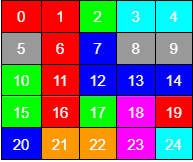
\includegraphics[scale=0.8]{./img/spread0.PNG}
    \end{center}
\end{figure}
Dès lors, les termes suivants seront utilisés pour décrire les aspects algorithmiques des fonctions que nous avons implémentés.
\begin{itemize}
    \item \textbf{Voisins d'une cellule :} Les voisins d'une cellule sont les cellules qui partagent un côté avec elle. (Exemple : les voisins de la cellule 0 sont \{1,5\}, les voisins de la cellule 6 sont \{1,5,7,11\})
    \item \textbf{Adjacence physique :} Deux cellules sont physiquement adjacentes lorsqu'elles sont voisines. (Exemple : Les cellules 0 et 5 sont physiquement adjacentes, les cellules 0 et 6 ne le sont pas)
    \item \textbf{Adjacence double :} Deux cellules sont doublement adjacentes si elles sont physiquement adjacentes et ont la même couleur. (Exemple : les cellules 0 et 1 sont doublement adjacentes, les cellules 0 et 6 ne le sont pas, les cellules 0 et 5 ne le sont pas). 
    \item \textbf{Partie connexe :} Est un ensemble de cellules connectées par double adjacence. (Exemple : les deux ensembles \{0,1,6,11,16\} et \{10,15\}sont deux parties connexes de tailles différentes)
    \item \textbf{Territoire d'un joueur:} Est la plus grande partie connexe contenant la position initiale du joueur. (Exemple : le territoire du premier joueur est \{0,1,6,11,16\}, le territoire du deuxième joueur est \{24\})
    \item \textbf{Frontière d'un joueur:} Est l'ensemble des cellules physiquement adjacentes au territoire du joueur. (Exemple : la frontière du premier joueur est \{5,10,15,21,17,12,7,2\}, celle du deuxième joueur est \{19,23\})
    \item \textbf{Frontière en profondeur:} Est l'ensemble des parties connexes dont l'une des cellules fait partie de la frontière du joueur. (Exemple : la frontière en profondeur du premier joueur est l'ensemble: \\ \{\{5\},\{10,15\},\{21,22\},\{17\},\{7,12,13,14\},\{2\}\})
\end{itemize}
La fonction \texttt{spread\_\_colors} que nous avons implémenté permet à un joueur d'étaler son territoire en changeant la couleur de ce dernier par la couleur passée en argument et c'est dans cette action que nous retrouvons l'utilité de la double adjacence discutée ci-dessus.\\
Nous mentionnons que \texttt{spread\_\_colors} représente une fonction intermédiaire servant à préparer les arguments d'une fonction récursive
\texttt{visit\_\_and\_color}. Ceci permet d'exploiter l'allocation automatique pour les variables auxiliaires nécessaires au processus de la propagation, cette méthode a été utilisée pour plusieurs autres fonctions afin d'éviter les déclarations des variables globales dans le serveur.\\
Voici un pseudo code décrivant le fonctionnement de \texttt{visit\_\_and\_color} :\\
\begin{lstlisting}
visit__and_color(cell: cellule, c: couleur du territoire,
                 colors: tableau de couleurs,
                 nv: nouvelle couleur) 
                 
    T = les voisins de cell
    pour chaque voisin x dans T
        si colors[x]==c
            colors[x] = nv
            visit__and_color(x, c, colors, nv)
\end{lstlisting}

La fonction \texttt{spread\_\_color} appelle la fonction décrite ci-dessus uniquement lorsque la couleur choisie par le joueur (donnée en argument) ne figure pas dans la liste des couleurs interdites. En pratique, la fonction renvoie 0 si la couleur choisie par le joueur est interdite et ne propage rien, dans le cas contraire la propagation est faite et la fonction renvoie 1.\\ 


Notons bien que le nombre d'appels récursifs lors de la propagation de couleur est limitée malgré le fait que la relation du voisinage est symétrique (potentiel d'une infinité d'appels entre deux cellules voisines lors d'un parcours en profondeur) car lors de chaque parcours nous changeons la couleur d'une cellule du territoire du joueur et par conséquent, celle-ci ne vérifiera pas la condition ( couleur de la cellule == couleur de la position initiale ) et donc n'engendrera pas un appel récursif. \\


Voici un exemple de 2 tours du jeu décrivant le fonctionnement de la fonction de propagation. 
\begin{figure}[htp]

\begin{subfigure}{0.3\columnwidth}
\centering
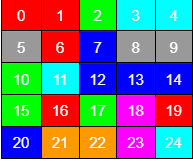
\includegraphics[width=\textwidth]{img/iteration1.PNG}
\caption{L'état de la grille initialement}
\label{fig:time1}
\end{subfigure}\hfill
\begin{subfigure}{0.3\columnwidth}
\centering
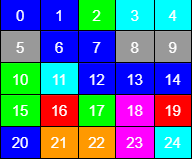
\includegraphics[width=\textwidth]{img/iteration2.PNG}
\caption{Le 1er joueur choisit bleu}
\label{fig:time2}
\end{subfigure}\hfill
\begin{subfigure}{0.3\columnwidth}
\centering
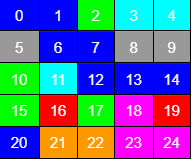
\includegraphics[width=\textwidth]{img/iteration3.PNG}
\caption{Le 2eme joueur choisit rose}
\label{fig:time3}
\end{subfigure}
\end{figure}
\newpage
\subsection{Calcul du score}
Comme mentionné avant, nous avons intérêt à calculer le score de chacun des deux joueurs à la dernière étape de la partie du jeu pour déclarer le joueur gagnant si personne des deux ne choisit une couleur interdite.\\


Par conséquent, nous avons implémenté une fonction \texttt{score\_\_of\_player} prenant en argument le graphe du jeu, l'ensemble des couleurs et un identifiant de joueur. Pour les mêmes raisons citées dans la partie précédente, cette fonction est une fonction intermédiaire qui alloue automatiquement les arguments nécessaires au calcul du score. Elle appelle la fonction \texttt{calculate\_\_score} qui a un comportement assez proche de la fonction de propagation puisqu'elle prépare les voisins de la cellule qu'elle prend en argument et incrémente une variable locale déclarée dans la pile de la fonction intermédiaire via son pointeur pris en argument.\\


De plus, la similarité ne s'arrête pas à cet aspect, puisque le calcul se fait par parcours en profondeur suite à un appel récursif sur chacun des voisins lorsqu'il appartient au territoire du joueur. \\Cependant, cette fois-ci, nous parcourons les cellules sans modifier leurs couleurs et par conséquent, nous devons marquer les cellules visitées pour limiter les appels récursifs, ceci est fait en passant à la fonction récursive un tableau "grey" de booléans. (grey[i]!=0 signifie que la cellule i a été visitée)\\

\subsection{Mise à jour des couleurs interdites}
Pour chacun des joueurs, en addition aux couleurs interdites fixées avant le début de la partie, il existe bien d'autres couleurs qui peuvent leurs être interdites et qui varient selon l'état de la grille du jeu comme mentionné dans la partie de description du jeu. Nous avons choisi de représenter ces couleurs par un tableau appelé forbidden dynamique et qui ressemble dans son implémentation au tableau forbidden invariable, une structure \texttt{color\_set\_t}:\\
\begin{lstlisting}
    struct color_set_t = {
        char t[MAX_COLOR];
        }
\end{lstlisting}
\\
La structure \texttt{color\_set\_t} contient un tableau de \texttt{char} qui représente la première lettre de la couleur. La quantité \texttt{MAX\_COLOR} représente le nombre total des couleurs possibles et qui a été fixé en 8 couleurs.\\

Chacun des joueurs n'a pas le droit de choisir une couleur qui ne lui apporte aucun point, ceci veut dire que nous avons besoin de retrouver la frontière de chacun des deux joueurs. Pour ce faire, nous avons implémenté une fonction \texttt{get\_Ctab\_neighbors} qui prend en argument le graphe, le tableau de couleurs, l'identifiant du joueur, la couleur du territoire du joueur ainsi que deux tableaux, l'un qui compte le nombre d'occurrences (initialement rempli par des 0 et dont la taille est égale au nombre de couleurs) d'une certaine couleur dans la frontière du joueur et un deuxième qui sert à marquer les cellules déjà visitées. Cette fonction prépare les voisins de la cellule en entrée dans un tableau, puis pour chacun des voisins, vérifie s'il a la même couleur du territoire (appartient à la frontière) ou non. Dans le cas où il appartiendrait à la frontière, il est marqué comme visité puis un appel récursif est fait en le prenant en argument (parcours en profondeur). Dans le cas contraire, si sa couleur est désignée par l'enter i, la fonction incrémente la i-ème position du tableau compteur d'occurrences des couleurs.\\


Ceci donc nous permet d'identifier une partie des couleurs interdites en cherchant le complémentaire de l'ensemble des couleurs de la frontière retrouvé par \texttt{get\_Ctab\_neighbors}.\\


Il existe un deuxième cas de couleurs interdites, c'est le cas où les deux territoires des joueurs sont connectés (c-à-d au moins l'une des cellules de la frontière du premier joueur est adjacente à au moins l'une des cellules de la frontière du deuxième joueur). Dans ce cas, chacun des joueurs n'a pas le droit de choisir la couleur de son adversaire. Voici une figure décrivant ce cas : 

\begin{figure}[h]
    \begin{center}
        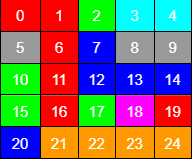
\includegraphics[scale=0.8]{./img/connected.PNG}
    \end{center}
\end{figure}
Nous remarquons que la cellule 16 du territoire du premier joueur est voisine à la cellule 21 du territoire du deuxième joueur, à cette étape, la couleur orange est interdite au joueur 1 et la couleur rouge est interdite au joueur 2. \\

Pour détecter une occurrence d'un tel cas dans nos parties du jeu, nous avons créé un ensemble de fonctions, chacune de ses fonctions avait sa propre utilité pour garantir le résultat final.\\



L'une des fonctions est la fonction \texttt{relatedComponentSmart} prenant en argument un graphe, le tableau de couleurs de la grille, une cellule, et un tableau vide. Cette fonction est responsable du remplissage du tableau en argument par la partie connexe du graphe qui contient la cellule en argument. Cette fonction est utilisée pour récupérer les frontières des deux joueurs puis les stocker dans deux tableaux déclarés automatiquement dans une fonction intermédiaire qui s'occupe de la phase suivante\\



Une fois que nos deux frontières sont fournies, il ne reste plus qu'à vérifier si il existe une cellule de la frontière du premier joueur qui est physiquement adjacente à l'une des cellules de la frontière du deuxième joueur. Pour ce faire, nous utilisons une troisième fonction prenant en argument le graphe du jeu et les deux tableaux contenant les deux frontières. Cette fonction effectue une première boucle sur l'ensemble des cellules de la première frontière et pour chacune de ces cellules, elle récupère les voisins dans un tableau local de taille 4. Ensuite, elle entre dans une deuxième boucle qui itère sur les cellules de la deuxième frontière, et pour chaque élément de cette frontière elle itère une dernière fois sur les éventuels 4 voisins de la cellule du premier joueur en question pour tester son adjacence à la cellule du deuxième joueur. Elle renvoie à la fin de son appel 1 lorsqu'il y a adjacence (les frontières sont connectées) sinon elle renvoie 0.\\


Grâce à la fonction décrite ci-dessus, nous avons pu détecter le cas de connexion entre les frontières des joueurs dans notre fonction de mise à jour des couleurs interdites et ainsi, nous ajoutons la couleur de l'adversaire dans le tableau forbidden dynamique.\\

\paragraph{Complexité des algorithmes : \\}
Nous avons remarqué que presque toutes les fonctions que nous venons de décrire s'appuient sur une même méthode algorithmique : le parcours en profondeur d'un graphe. Dans notre cas, le parcours ne se fait que sur les graphes représentés par les territoires des joueurs et qui sont d'ailleurs rarement de l'ordre du nombre de cellules (Ça ne peut se produire que si l'un des deux joueurs ne fait que passer sont tour, ie. choisir \texttt{NO\_COLOR}). Dans le cas de la fonction \texttt{visit\_\_and\_color} par exemple, le nombre de sommets concernés par un parcours est dans le pire des cas à peu près égale au nombre des cellules de la grille qu'on notera n. Dans la fonction de propagation, les instructions se limitent à la récupération des voisins de la cellule de l'entrée, chose qui est faite en un temps constant grâce à la factorisation des matrices d'adjacence, et le changement de couleur de la cellule (ou non) qui se fait également en temps constant. Sachant que le nombre d'appels maximale est égal à n, nous déduisons que la complexité temporelle de la fonction de propagation est linéaire. En addition, puisque le calcul du score ainsi que la mise-à-jour des couleurs interdites suivent à peu près la même démarche algorithmique que celle de la propagation des couleurs, nous déduisons que la complexité temporelle de ces fonctions est également linéaire.



\noindent
%Cette complexité est la même pour les trois autres fonctions citées ci-dessus également. Bien que leurs objectifs, prototype et attentes soient différents, le parcours en profondeur est le trait commun qui relie entre ces fonctions. Ceci souligne l'utilité et l'importance de ce type de parcours ainsi que la simplicité et l'efficacité de la représentation du jeu par un graphe.



\subsection{stratégies}



\paragraph{Le joueur aléatoire :\\}




Représente notre premier joueur implémenté, il joue une couleur aléatoire non-présente dans le tableau des couleurs non permises (\textt{Forbidden\_colors}), si aucune couleur ne lui est permise, il joue \texttt{NO\_COLOR}.\\



\paragraph{Couleur maximale : \\}



C'est une stratégie qui permet au joueur d'effectuer un coup en se basant sur le tableau get\_Ctab\_neighbors, en choisissant la couleur qui a le plus d'occurrences dans la frontière du joueur.
.\\
\begin{figure}[!h]
\begin{center}
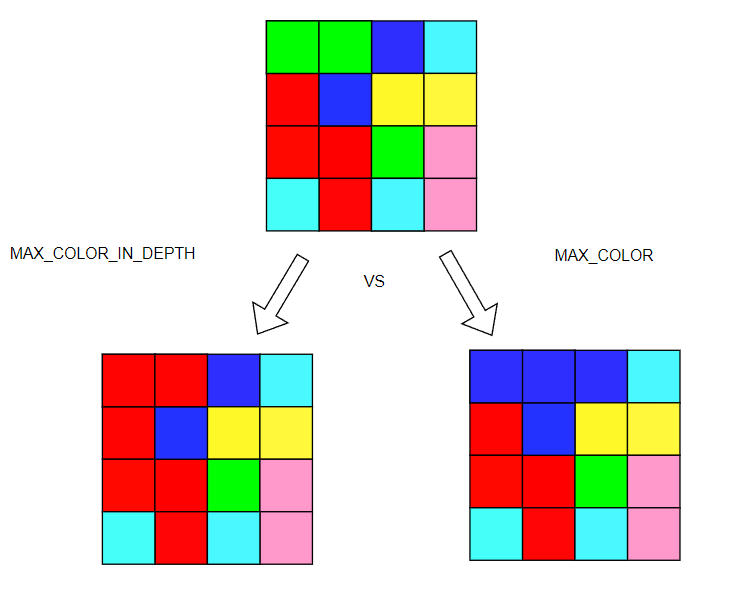
\includegraphics[scale=0.7]{./img/graph_depth2.png}
\caption{Max\_Color\_In\_Depth vs Max\_Color }
\label{fig: 6}
\end{center}
\end{figure}

\paragraph{Couleur maximale en profondeur :\\}
En un coup, une couleur peut mieux étaler le territoire du joueur sans qu'elle ne soit prédominante dans la frontière.\\
C'est pour cela qu'on implémente une fonction \texttt{get\_Ctab\_neighbors\_smart} qui fournit un tableau contenant le nombre d'occurrences de chaque couleur en profondeur à partir de la frontière du joueur.\\
Pour le joueur 1 dans la figure \ref{fig: 6}, \texttt{get\_Ctab\_neighbors\_smart} nous fournit un tableau avec la couleur rouge 4 fois itérée et la couleur bleue 2 fois itérée tandis que \texttt{get\_Ctab\_neighbors} donne un tableau d'occurrence des couleurs: (bleu=2,rouge=1), le coup permettant de mieux propager son territoire est fourni par le premier tableau .\\


Cette fonction utilise un raisonnement similaire à \texttt{get\_Ctab\_neighbors}, un parcourt en profondeur de la même manière pour obtenir les cellules de la frontière, il suffit ensuite d'appliquer la fonction \texttt{relatedComponentSmart} sur chaque élément pour obtenir les parties connexes de chaque composante dans la frontière. \\Deux cellules de la frontière appartenant à la même partie connexe risquent d'être prises en compte deux fois, pour y remédier, on marque chaque cellule visitée de la partie connexe fournie par \texttt{relatedComponentSmart}. \\Avec les cellules de la frontière\_en\_profondeur, on obtient le nombre d'occurrences de chaque couleur qui nous donne le \texttt{MAX\_COLOR\_IN\_DEPTH}. \\

\paragraph{Best moves\_in\_advance : \\}
En précisant le nombre (\texttt{num}) de coups qu'on veut prévoir en avance, cet algorithme permet d'avoir les coups qui maximisent le score après \texttt{num} coups de le début de partie, c'est la fonction \texttt{moves\_in\_advance} qui permet d'aboutir à ce résultat.\\
Le principe de cette stratégie est de simuler des éventuelles séquences de \texttt{num} coups permis dans une grille virtuelle pour ensuite choisir la meilleure combinaison maximisant le territoire du joueur.\\
On appelle la fonction avec le tableau de couleur initiale du joueur et les couleurs qui lui sont permises, un tableau \texttt{move\_dynamic} de la taille des coups attendus \texttt{num}, qui sera remplie à fur à mesure avec les coups de taille \texttt{num} qui permettent au joueur de conquérir un maximum de cellule au début du jeu. \\
Un autre tableau de coups (\texttt{move\_static}) sera fourni pour stocker les coups intermédiaires de taille inférieure à \texttt{num} et à chaque appel de la fonction, on effectue des copies du tableau de couleur et du tableau des coups \texttt{move\_static}, on les modifie puis on prend pour le prochain appel de fonction ces nouveaux paramètres qui décrivent le nouvel état après avoir propagé une couleur permise sur la grille "virtuelle" du joueur.\\

On calcule le score de chaque combinaison de coup de taille \texttt{num} et on affecte à \texttt{move\_dynamic} celle qui fournit le plus grand score.\\
La taille des grilles est prise en compte dans le choix de \texttt{num}. Par exemple pour une grille de taille \texttt{10x10} on prend $\texttt{num}=5$. Cette valeur nous permet de toujours prendre l'avantage au début de la partie. Le joueur termine ensuite la partie avec l'algorithme du \texttt{MAX\_COLOR\_IN\_DEPTH}. Cette stratégie nous a permis de décrocher la première place au ladder. En sachant que le joueur implémentant la stratégie du \texttt{MAX\_COLOR\_IN\_DEPTH} est $5^{eme}$ sur ce ladder.

\begin{figure}[h!]
\begin{center}
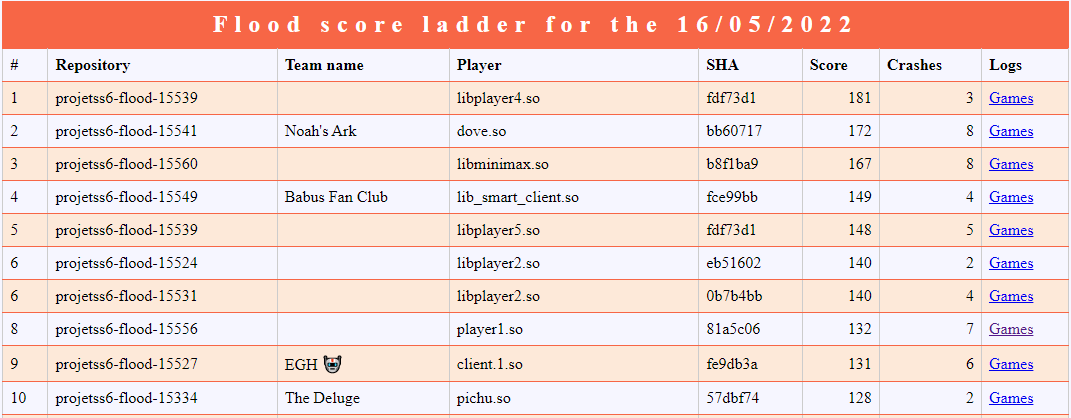
\includegraphics[scale=0.45]{./img/ladder.PNG}
\end{center}
\end{figure}

\paragraph{Complexité de la fonction moves\_in\_advance : \\}
Cette complexité est illustrée sur la figure \ref{fig:7}, on suppose que que 4 couleurs existent dans le jeu {bleu, jaune, rouge, vert}, donc il a le droit d'en choisir trois à chaque tour.\\
Au début, le joueur possède la couleur bleue puis en prenant dans notre exemple $num=2$, on obtient sur les 2 coups en avance qu'il prévoie,  $3^3$ appels de la fonction spread et $3^2$ appel de la fonction score pour choisir la combinaison de deux coups avec le meilleur score .\\
Donc la complexité de moves\_in\_advance est dans le pire des cas si on a toujours $Max\_Num\_colors-1$ sur la frontière du joueur, en posant\\ M=($Max\_Num\_colors-1$) on obtient pour la complexité:\\ $M^{num+1}$$\times$$complexity(spread)$+$M^{num}$$\times$$complexity(score)$
\\
Donc la complexité avec N le nombre de sommets est : $O(M^{num+1}\times{N})$

\begin{figure}[h!]
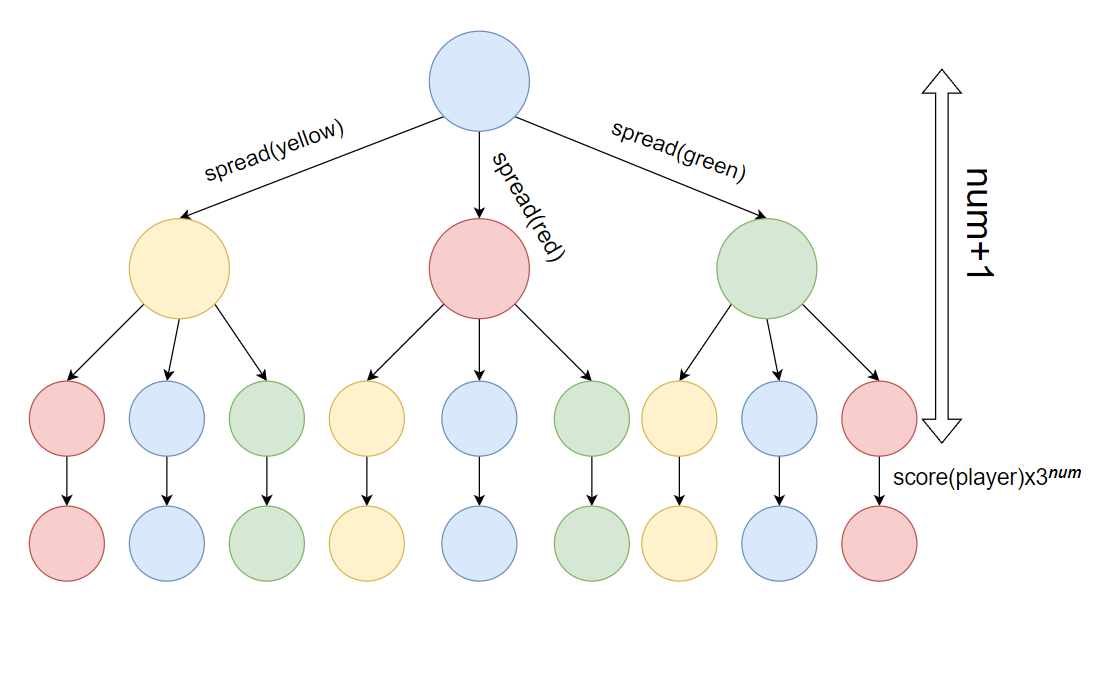
\includegraphics[scale=0.6]{./img/move_in_advance.png}
\caption{complexité de moves\_in\_advance dans un cas particulier}
\label{fig:7}
\end{figure}
\newpage

\section{tests et validation}
La partie la plus importante du projet concerne les tests effectués pour valider les résultats des fonctions. En particulier, celles qui jouent un rôle fondamental dans la propagation des couleurs et l'exécution de nos stratégies. Afin de vérifier que notre programme fonctionne correctement et dans un premier temps, on a réalisé des parties entre différentes stratégies et d'un autre côté, nous avons effectué des tests unitaires pour les fonctions importantes en prenant compte des cas limite qui puissent poser des problèmes.
\subsection{Exemples de partie entre stratégie}
 Nos joueurs \texttt{p1}, \texttt{p2} et \texttt{p3} utilisent des stratégies différentes et d'après nos implémentations \texttt{p1} est censé gagner contre \texttt{p2} et \texttt{p3},et \texttt{p2} doit gagner contre \texttt{p3}.\\
 Alors, afin de vérifier cette hiérarchie, prenant comme test les parties disponibles sur le ladder : \\
\begin{figure}[h!]
    \centering
    \begin{minipage}[c]{.46\linewidth}
        \centering
        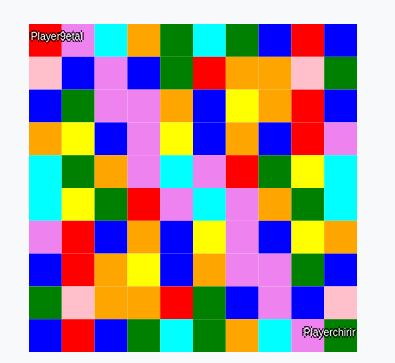
\includegraphics[scale=0.3]{img/9etal_vs_chirir.png}
    \end{minipage}
    $\longrightarrow$
    \begin{minipage}[c]{.46\linewidth}
        \centering
        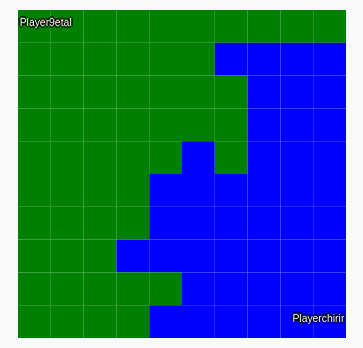
\includegraphics[scale=0.3]{img/9etal_vs_chirir_end.png}
    \end{minipage}
    \caption{\texttt{p1 vs p2 : 56 vs 44}}
\end{figure}


\begin{figure}[h!]
    \centering
    \begin{minipage}[c]{.46\linewidth}
        \centering
        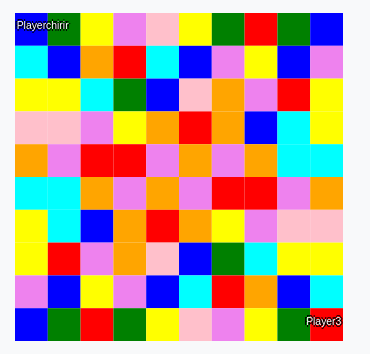
\includegraphics[scale=0.3]{img/3_vs_chirir.png}
    \end{minipage}
    $\longrightarrow$
    \begin{minipage}[c]{.46\linewidth}
        \centering
        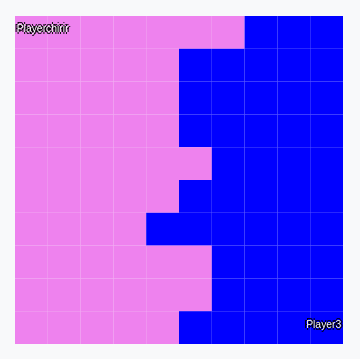
\includegraphics[scale=0.3]{img/3_vs_chirir_end.png}
    \end{minipage}
    \caption{\texttt{p2 vs p3: 54 vs 46}}
\end{figure}

En effet, le score de chaque partie et l'écart entre les scores de chaque joueur montre effectivement la hiérarchie entre les stratégies en terme de puissance.

\subsection{Tests}
Les tests ont été choisis en prenant en considération les différents types de graphes, de colorations, de cas limite de la propagation de couleurs et des calculs d'occurrences aux frontières. La vérification des résultats est effectuée grâce à la fonction \texttt{assert} de la bibliothèque assert.h .
\begin{itemize}
\item Les premiers tests concernent la génération des graphes et des couleurs dans le fichier \texttt{test\_graph.c}. Pour cela, on a effectué quatre tests, un pour chaque type de graphe, en choisissant un type de générateur de couleurs de notre choix pour chaque test.

\item Les tests suivant sont ceux de la fonction \texttt{get\_Ctab\_neighbors}. Elle se distingue par son utilisation dans une stratégie et aussi par son rôle dans la propagation des couleurs. En fixant la coloration cyclique, ses fonctions de tests se basent sur deux choses : la position du joueur (0 ou $n^{2}-1$) et le type du graphe.

\item Les tests qui permettent de propager les couleurs sont effectués de la même manière que ceux de \texttt{get\_Ctab\_neighbors}, en ajoutant des tests sur les changements des tableaux \texttt{forbidden} avant et après la propagation.
\end{itemize}

\section{Conclusion}
\subsection{Résultat final}
Durant ce projet, nous étions capables de créer le jeu de flood-filling en simulant une partie entre différents joueurs et stratégies de jeux.\\
Cependant, il était possible d'améliorer certains points et de perfectionner nos algorithmes ainsi que d'ajouter d'autres formes de graphes en ajoutant des obstacles (une autre couleur, le noir par exemple) bloquant la propagation des joueurs.

Néanmoins, quelques points ont posé plusieurs problèmes:
\begin{itemize}
\item Le problème de considérer et de gérer des couleurs interdites dynamiques et statiques, des couleurs qui sont interdites durant toute la partie et des couleurs qui changent après chaque propagation.
\item Le débogage des erreurs qui parfois n'apparaissent que lors des parties avec d'autres serveurs.
\end{itemize}
\subsection{Bilan personnel}
Ce projet nous a permis de mettre en application nos connaissances en C (création d'un \texttt{Makefile}, des bibliothèques partagées et le débogage avec \texttt{GDB}), ainsi que nos connaissances algorithmiques en général (avec l’implémentation de quelques algorithmes de graphes).
Nous avons aussi appris à travailler en équipe sur un projet de programmation tout en partageant plusieurs tâches. Notamment : apprendre à utiliser \textt{GIT} pour partager son code, découper et se répartir le travail et s’entraider.

\end{document}
